\documentclass{beamer}
\usetheme{Boadilla}
\usepackage{ifpdf}
\ifpdf
\usepackage[utf8]{inputenc}
\usepackage[T1]{fontenc}
\usepackage[all,pdf,2cell]{xy}\UseAllTwocells\SilentMatrices
\else
\usepackage[all,xdvi,2cell]{xy}\UseAllTwocells\SilentMatrices
\fi

\usepackage{newunicodechar}
\usepackage{cmbright}

\newtheorem{proposition}[theorem]{Proposition}
\newcommand{\id}{\mathrm{id}}
\newcommand{\obj}{\mathrm{obj}}
\newcommand{\C}{\mathcal{C}}
\newcommand{\D}{\mathcal{D}}
\newcommand{\isleftadjoint}{\dashv}
\newcommand{\VoltG}{{\mathbf{Volt}_Γ}}
\newcommand{\LabG}{{\mathbf{Lab}_Γ}}
\newcommand{\ActLab}{{\mathbf{ActLab}_Γ}}
\newcommand{\KG}{{\mathring{K}(Γ)}}
\newcommand{\K}{\mathring{K}}
\renewcommand{\k}{\mathring{k}}
\newcommand{\lG}{{\ell(Γ)}}
\newcommand{\pb}[3]{{#1}×_{#2}{#3}}
\newcommand{\newcategory}[1]{\expandafter\newcommand\csname #1\endcsname{\mathbf{#1}}}
\newcommand{\Graph}{\mathbf{Graph}}
\newcommand{\Volt}{\mathbf{Volt}}
\newcommand{\Lab}{\mathbf{Lab}}

\newunicodechar{α}{\alpha}
\newunicodechar{β}{\beta}
\newunicodechar{λ}{\lambda}
\newunicodechar{Γ}{\Gamma}
\newunicodechar{×}{\times}

\title[Derived graphs]{Derived graphs come from an adjunction\\
\small{arXiv:????}}
\author{Gejza Jenča}
\institute[]{Slovak University of Technology Bratislava}
\date{\today}

\begin{document}
\begin{frame}
\maketitle
\end{frame}
\begin{frame}
\frametitle{Graphs}
A {\em graph} is a quadruple $G=(V,D,s,t,λ)$, where
\begin{itemize}
\item $D$ is the {\em set of darts of $G$}
\item $V$ is the {\em set of vertices of $G$}
\item $s,t\colon D\to V$ are the {\em source and target maps}, respectively.
\item $λ\colon D\to E$ is a mapping such that $λ\circλ=\id_D$.
\item $s\circλ=t$.
\end{itemize}
The mapping $λ$ is called the {\em dart-reversing involution} of $G$.
\end{frame}
\begin{frame}
\frametitle{Graphs}
All the data in a graph $(V,D,s,t,λ)$ can be expressed graphically by a commutative diagram:
\begin{equation}
\xymatrix{
D
	\ar@/^/[rr]^{\id_D}
	\ar[rd]^{λ}
	\ar@/_/[rdd]_{s}
&
~
&
D
	\ar@/^/[ldd]^{s}
\\
~
&
D
	\ar[d]^-{t}
	\ar[ru]^{λ}
\\
~
&
V
}
\label{diag:G}
\end{equation}

\end{frame}
\begin{frame}
\frametitle{Morphisms of graphs}
A {\em morphism of graphs} $f\colon G\to H$ is a pair of mappings $(f^V,f^D)$, where 
\begin{itemize}
\item $f^V\colon V(G)\to V(H)$
\item $f^D\colon D(G)\to D(H)$
\item for every dart $d\in D(G)$
\begin{align*}
s(f^D(d))&=f^V(s(d))\\
t(f^D(d))&=f^V(t(d))\\
λ(f^D(d))&=f^D(λ(d))
\end{align*}
\end{itemize}

Clearly, graphs equipped with morphisms form a category, denoted by $\Graph$. 
\end{frame}

\begin{frame}
\frametitle{Voltage graphs}

A {\em voltage graph} is a triple $(G,Γ,α)$,
where 
\begin{itemize}
\item $G$ is a graph
\item $Γ$ is a group
\item $α\colon D(G)\to Γ$ is a mapping such that 
$$α(λ(d))=(α(d))^{-1}$$
\end{itemize}
The mapping $α$ is called a {\em $Γ$-voltage on $G$}.
\end{frame}
\begin{frame}
\frametitle{Derived graph}
\begin{definition}\cite{gross2001topological}
\label{def:derived} 
Let $(G,Γ,α)$ be a voltage graph. There is a {\em derived $Γ$-voltage graph of
$(G,Γ,α)$},
denoted by $(G^α,Γ,α')$
\begin{itemize}
\item $V(G^α)=V(G)×Γ$
\item $D(G^α)=D(G)×Γ$
\item $s(d,x)=(s(d),x)$
\item $t(d,x)=(t(d),x.α(d))$
\item $λ(d,x)=(λ(d),x.α(d))$
\item $α(d,x)=α(d)$
\end{itemize}
\end{definition}
\end{frame}
\begin{frame}
\frametitle{An example; the group is $\mathbb Z_3$}
\begin{center}
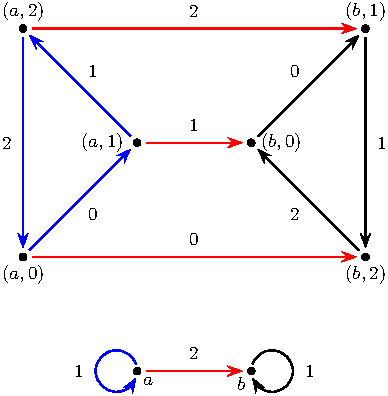
\includegraphics[scale=0.8]{derived1}
\end{center}
\begin{itemize}
\item There is always a projection map: $((a,x)\mapsto a)\colon G^α\to G$
\item The projection map is a very nice surjection (a {\em covering}).
\end{itemize}
\end{frame}
\begin{frame}
\frametitle{Morphisms of voltage graphs}

A morphism of voltage graphs $(G,Γ,α)\to(G',Γ',α')$ is a pair $(f,h)$,
where 
\begin{itemize}
\item $f\colon G\to G'$ is a morphism of graphs
\item $h\colon Γ\to Γ'$ is a morphism of groups such that,
\item for all $d\in D(G)$, $h(α(d))=α'(f^D(d))$.
\[
\xymatrix{
D(G)
	\ar[r]^{f^D}
	\ar[d]_\alpha
&
D(G')
	\ar[d]^{\alpha'}
\\
\Gamma
	\ar[r]_h
&
\Gamma'
}
\]
\item The category of voltage graphs is denoted by $\Volt$.
\end{itemize}

\end{frame}
\begin{frame}
\frametitle{Group labeled graphs}

A {\em group labeled graph} 
is a triple $(G,Γ,β)$,
where $G$ is a graph, $Γ$ is a group and $β\colon V(G)\to Γ$ is a mapping, called a {\em $Γ$-labeling on
$G$}.

\end{frame}
\begin{frame}
\frametitle{Morphisms of group labeled graphs}
A morphism of group labeled graphs $(G,Γ,β)\to (G',Γ',β')$ is a
pair $(f,h)$, where 
\begin{itemize}
\item $f\colon G\to G'$ is a morphism of graphs
\item $h\colon Γ\to Γ'$ is a morphism of groups
\item for all $v\in V(G)$, $h(β(v))=β'(f^V(v))$.
\[
\xymatrix{
V(G)
	\ar[r]^{f^V}
	\ar[d]_\beta
&
V(G')
	\ar[d]^{\beta'}
\\
\Gamma
	\ar[r]_h
&
\Gamma'
}
\]
\item The category of group labeled graphs is denoted by $\Lab$.
\end{itemize}
\end{frame}
\begin{frame}
\frametitle{From group labeled graphs to voltage graphs}

For every group labeled graph $L(G,Γ,β)$, there is a voltage graph
$L(G,Γ,β)=(G,Γ,α)$, with the voltage $α$ given by the rule
$α(d)=β(s(d))^{-1}β(t(d))$.
\begin{center}
\includegraphics{left}
\end{center}
$L$ is a functor $\Lab\to\Volt$.
\end{frame}
\begin{frame}
\frametitle{Main results}
\begin{itemize}
\item
There is an adjunction
$$
\xymatrix{
\Lab
	\ar@/^1.2pc/[rr]^-L
&
\bot
&
\Volt
	\ar@/^1.2pc/[ll]^-R
}
$$
between a category  $\Volt$ of voltage graphs and a
category $\Lab$ of group labeled graphs. 
\item For every voltage graph $(G,Γ,α)$,
$LR(G,Γ,α)$ is the derived voltage graph.
\item
The canonical projection
$LR(G,Γ,α)\to(G,Γ,α)$ is the counit of the $L\isleftadjoint R$ adjunction.
\end{itemize}
\end{frame}
\end{document}
